\chapter{Performance of Our Driver: Results and Discussion}
\label{chap:performance}
To compare the performance of our driver to BitLocker and VeraCrypt, we conducted several experiments measuring the read rates for both sequential and random access. Preliminary tests were done in a virtual machine, and after some optimizations, we tested more extensively on real hardware. Finally, we also measured how the read rates behave over time.

\todo{\autoref{app:onlinereferences} describes how to obtain copies of the data collected in our measurements. It also links to a Git repository containing the code that generated the figures presented in this section.}

\section{Experimental Setup}
\label{chap:performance.setup}
Both the setup for the virtual machine and the real hardware will be described in this section. They are mostly the same, so unless stated otherwise, the contents in this section apply to both.

Both configurations used a fresh Windows 10 build 19043.928 install. The virtual machine ran in Oracle VirtualBox 6.1.22 with 8 GiB of virtual RAM (backed by 16 GiB DDR4 RAM), 4 virtual cores (backed by a Intel Core i7-7700K), and two virtual disks (backed by a 250 GB Samsung SSD 850 EVO). The real machine had 8 GiB DDR3 RAM, an Intel Core i7-3770 quad core with simultaneous multithreading, and a 233 GiB SanDisk SDSSDH3250G.

For each encryption technique featured in our benchmarks we created a separate 5 GiB FAT32 volume on the same disk, as shown in \autoref{fig:performance.setup.disklayout}. Every encrypted volume contained the same file, \texttt{random.bin} (4 GiB of random data). We configured BitLocker to use the new AES-XTS mode, all other settings were left unchanged. For VeraCrypt, we also used AES-XTS with SHA-256 and also mounted the volume as read-only after copying the \texttt{random.bin} file to it.

\begin{figure}[htb!]
	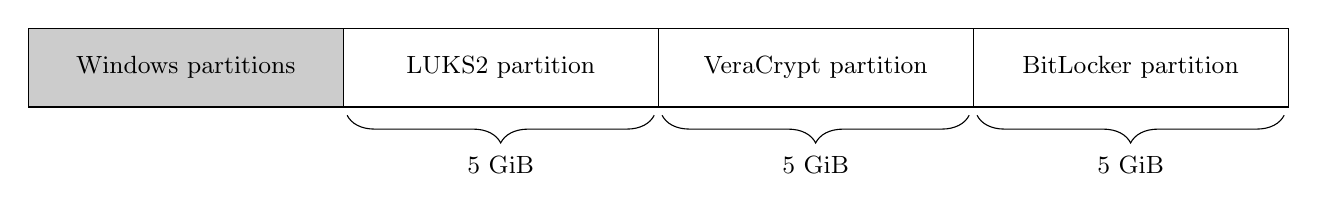
\begin{tikzpicture}
		\draw [fill={gray!40}] (0, 0) rectangle (4, 1);
		\node [anchor=center] at (2, 0.5) {\small\makecell{Windows partitions}};
		\draw [fill=white] (4, 0) rectangle (8, 1);
		\node [anchor=center] at (6, 0.5) {\small\makecell{LUKS2 partition}};
		\draw [fill=white] (8, 0) rectangle (12, 1);
		\node [anchor=center] at (10, 0.5) {\small\makecell{VeraCrypt partition}};
		\draw [fill=white] (12, 0) rectangle (16, 1);
		\node [anchor=center] at (14, 0.5) {\small\makecell{BitLocker partition}};

		\draw [decorate, decoration={brace, amplitude=10pt, mirror}, yshift=-3pt]
		(4.05, 0) -- (7.95, 0) node [black, midway, yshift=-18pt] {\small 5 GiB};
		\draw [decorate, decoration={brace, amplitude=10pt, mirror}, yshift=-3pt]
		(8.05, 0) -- (11.95, 0) node [black, midway, yshift=-18pt] {\small 5 GiB};
		\draw [decorate, decoration={brace, amplitude=10pt, mirror}, yshift=-3pt]
		(12.05, 0) -- (15.95, 0) node [black, midway, yshift=-18pt] {\small 5 GiB};
	\end{tikzpicture}
	\caption[
		Volume layout for our experiments
	]{
		Volume layout for our experiments. This is the layout of the real hardware SSD. The virtual machine had a virtual disk for the Windows installation and another one for the three encrypted volumes.
	}
	\label{fig:performance.setup.disklayout}
\end{figure}

To compare the performance of the different drivers, we used version 3.27 of the \texttt{fio} command line tool \cite{Fio} to read from the three copies of \texttt{random.bin}, using different access patterns. Each run of \texttt{fio} is called a \emph{job}, and the configuration for a job is stored in a \emph{job file}. We maintained a different job file for each of the three encryption technologies. \autoref{fig:performance.setup.fiojobfile} describes the different parameters that we used and shows the configuration for \texttt{luks2flt}. \texttt{fio} allows the user to specify which I/O engine to use. The default on Windows is the native asynchronous I/O API, which is what we used.

\begin{figure}[htb!]
	\begin{inicode}
[luks2flt]
filename=L\:\random.bin
thread
iodepth=${IODEPTH}
numjobs=${NUMJOBS}
rw=${MODE}
bs=${BLOCKSIZE}
	\end{inicode}
	\caption[
		\texttt{fio} job file for \texttt{luks2flt}
	]{
		\texttt{fio} job file for \texttt{luks2flt}. It defines one job called \texttt{luks2flt}. The \texttt{filename} option's value is the only one that depends on the used driver; the rest of the configuration is the same for BitLocker and VeraCrypt. The \texttt{thread} option means that \texttt{fio} will create threads instead of processes to run jobs (which is always done on Windows, but when not specifying this option, the user is warned about this behaviour). The \texttt{iodepth} parameter controls how many I/O operations \texttt{fio} will try to submit before waiting for the completion of submitted requests (i.e. the size of the internal queue of submitted I/O requests). \texttt{numjobs} controls how many threads will concurrently execute the job (note that each thread does a full run of the job, i.e. each thread reads the complete file and has its own queue with the size specified by \texttt{numjobs}). \texttt{rw} holds the access mode, in our case it is always \texttt{read} (sequential reading) or \texttt{randread} (random-access reading). The blocksize of read operations, i.e. how the number of bytes read in a single I/O operation, is given by the \texttt{bs} option. All parameter values of the form \texttt{\$\{PARAM\}} are configured by environment variables \cite{Fio}.
	}
	\label{fig:performance.setup.fiojobfile}
\end{figure}

We also looked at other I/O benchmarking programs, but found that they all required write access. This unfortunately made them unfit for our cause.

We wrote a PowerShell script to automate running jobs with different parameters. Its task was to set the environment variables used in the job files to their respective values and to invoke \texttt{fio}, pointing it to the correct job file. A sample invocation looks like this: \texttt{fio ---readonly ---output-format=json ---output luks2flt.json luks2flt.fio}. The \texttt{---readonly} option is necessary because even though we only specified read operations, execution would fail for read-only volumes. The data visualized by the graphs in the following sections was taken from \texttt{fio}'s JSON output.

\section{Virtual Machine Experiments}
\label{chap:performance.vmexperiments}
To get a first impression of \texttt{luks2flt}'s performance, we ran a first series of experiments in a virtual machine.\footnote{\label{fn:performance.vmexperiments.vm} Note that this virtual machine had not been started in debug mode and was not connected to a WinDbg kernel debugging session, so as to not impact performance.} These experiments were only conducted once, which leaves room for variation in read rates. Therefore the results in this section need to be taken with a grain of salt. We will address this issue in \autoref{chap:performance.hwexperiments}.

When we looked at the results of our measurements, we were convinced that there was still some optimization possible. We first checked the compiler's optimization settings, and found that the default compiler optimization settings in Visual Studio were a bit conservative. They were also set to optimize for small code size rather than high speed/performance. We therefore tuned these settings to enable more aggressive optimizations and also focus on speed rather than code size. This led to a more optimized version of \texttt{luks2flt}. The results presented in this section feature both the first and the more optimized version.

\paragraph{Results and Observations}
\autoref{fig:performance.vmexperiments.seq} shows a comparison of the read rates for sequential access, with block sizes ranging from 4 to 8192 KiB. The featured drivers are BitLocker, VeraCrypt and the two versions of \texttt{luks2flt} (before and after enabling more optimizations). BitLocker consistently has the highest read rate, starting at 171 MiB/s for 4 KiB blocks, rising with bigger blocks, until peaking at 469 MiB/s for a block size of 4096 KiB. VeraCrypt generally has the second-highest rate, starting at 154 MiB/s, with an upwards trend until the maximum of 341 MiB/s is reached for 256 KiB blocks. It then slowly falls back down to 329 MiB/s. The optimized \texttt{luks2flt} version comes third, starting at 144 MiB/s and rising to 344 MiB/s, beating VeraCrypt at the largest block size. \texttt{luks2flt}'s less optimized variant always has the lowest read rate, beginning at 119 MiB/s and climbing to 217 MiB/s.

\begin{figure}[htb!]
	\center
	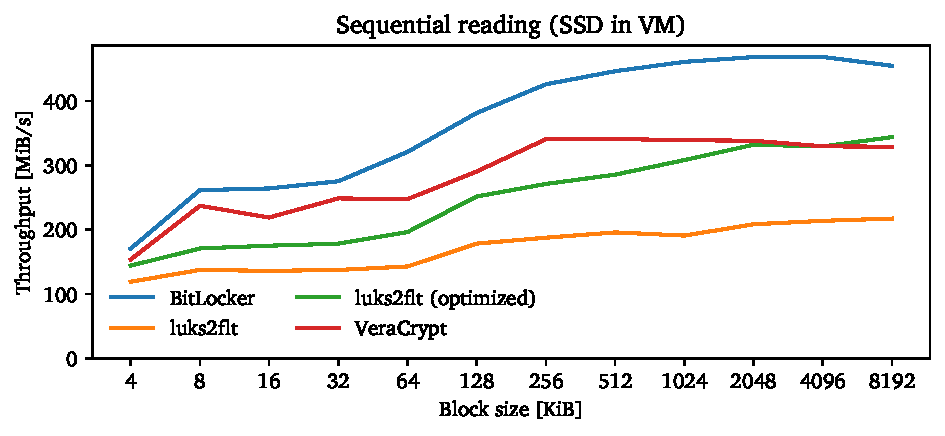
\includegraphics[scale=1]{../fig/performance.vmexperiments.seq.pdf}
	\caption[
		Sequential read rates in the virtual machine
	]{
		Sequential read rates in the virtual machine. The data was obtained by running jobs back to back: one job per combination of driver and block size, grouped by driver and ordered by increasing block size. There was a reboot after the BitLocker, VeraCrypt, and optimized \texttt{luks2flt} jobs to load the less optimized version of \texttt{luks2flt}. Both the \texttt{iodepth} and \texttt{numjobs} parameters were set to a value of 1.
	}
	\label{fig:performance.vmexperiments.seq}
\end{figure}

% the high beginpenalty (oftend used in the rest of this chapter) prevents a page break occurring between the line of text and the first item
We observe the following:
\begin{itemize}[beginpenalty=10000]
	\item BitLocker's sequential read rate is greater than our driver's and VeraCrypt's for all tested block sizes.
	\item VeraCrypt performs noticeably better at sequential reading than \texttt{luks2flt}'s optimized version, but the difference decreases with increasing block size. VeraCrypt's read rate peaks at 256 KiB, but our driver's rate continues to grow after that.
	\item The more optimized version has a significantly higher sequential read rate than the first version, especially at larger block sizes. At 4 KiB, the increase in performance is about 21\%; at 8192 KiB the more optimized version has about a 59\% higher read rate.
\end{itemize}

\autoref{fig:performance.vmexperiments.rand} shows the random access read rates of the four drivers for different block sizes. BitLocker always has the highest rate, starting at 16 MiB/s and climbing up to 388 MiB/s at 8192 KiB blocks, with a little stagnation and decrease in performance at 256 and 512 KiB. VeraCrypt has the lowest read rate of 10 MiB/s at 4 KiB, but it steadily grows: it rises to third place at 256 KiB, second place at 1024 KiB, and falls back to third at 8192 KiB, with a maximum of 291 MiB/s. The two versions of \texttt{luks2flt} both start at 16 MiB/s and rise for block sizes up to 128 KiB, switching their roles of second and third place. After that, the optimized version continues to improve its read rate up to the final value of 300 MiB/s, temporarily falling behind VeraCrypt. The less optimized version's rate first decreases a bit, then rises abruptly, and then decreasing a bit again, with a maximum value of 144 MiB/s at 1024 KiB.

\begin{figure}[htb!]
	\center
	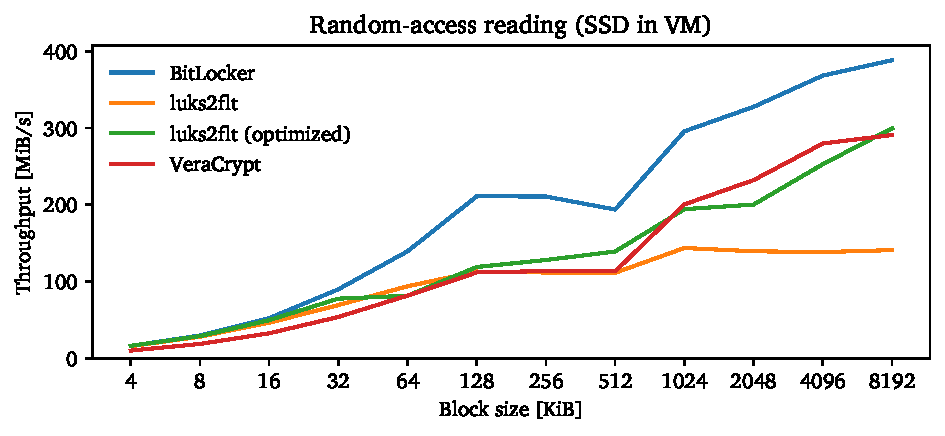
\includegraphics[scale=1]{../fig/performance.vmexperiments.rand.pdf}
	\caption[
		Random-access read rates in the virtual machine
	]{
		Random-access read rates in the virtual machine. See \autoref{fig:performance.vmexperiments.rand} for how we collected the data.
	}
	\label{fig:performance.vmexperiments.rand}
\end{figure}

We observe the following:
\begin{itemize}[beginpenalty=10000]
	\item BitLocker has the highest random-access read rate, with sometimes almost double the rate of the others (e.g. at 128 KiB).
	\item The optimized version of \texttt{luks2flt} beats VeraCrypt's random-access read rate at two thirds of the tested block sizes. For example, its read rate is 60\% higher at 4 KiB, 52\% higher at 16 KiB, and 14\% lower at 2048 KiB.
	\item Starting from a block size of 128 KiB, the more optimized version has a significantly higher random-access read rate than the first version. For the biggest block size, the more optimized version has a 113\% higher read rate.
\end{itemize}

\paragraph{Discussion}
Combining our observations from both access patterns, we close with the following thoughts:
\begin{itemize}[beginpenalty=10000]
	\item BitLocker is the best-performing driver, both at sequential and random-access reading. This is not really surprising, as it is not a fair competition: one driver is the proprietary product of Microsoft, who also wrote the operating system running the driver; and the other two are open source projects by third parties. Microsoft's driver profits from their expertise in Windows' inner workings, and can also take advantage of undocumented internals.
	\item VeraCrypt has a higher sequential read rate than \texttt{luks2flt}, with the difference decreasing for larger block sizes. The former is probably because of VeraCrypt's read ahead caching, as \texttt{luks2flt} does not perform any caching. The latter may be because of VeraCrypt's fragmenting of larger blocks into 256 KiB blocks. This means that the I/O performed by the driver can only profit so much from block sizes larger than 256 KiB. This theory is supported by the fact that VeraCrypt reaches its peak sequential read rate at exactly this block size. As already mentioned in \autoref{chap:otherapproaches.veracrypt.peeking}, the fragmenting is done to overlap I/O and cryptographic operations. However, the alleged gains from this overlapping do not seem to be able to cancel out the losses by capping the effective block size at 256 KiB.
	\item For random-access reads, the performance difference between VeraCrypt and \texttt{luks2flt} is smaller, with our driver showing higher read rates most of the time. This supports the thesis that VeraCrypt's performance advantage for sequential access stems from its caching: for random access reads the cache is not effective, and therefore the advantage vanishes.
	\item The changed compiler optimization settings have a significant impact on our driver's read performance, regardless of the access pattern.
\end{itemize}

\paragraph{Another Optimization Attempt}
We also tried optimizing \texttt{luks2flt}'s performance by restricting its cryptographic capabilities to AES-256-XTS and dropping support for AES-128-XTS. This enabled removing some \texttt{if}-\texttt{else} constructs that dispatched de-/encryption functions based on whether AES-128 or AES-256 was used. Even though these conditionals were located in a performance critical section, we found no significant read rate changes. Our theory for why this was the case is the following: in this setup, our driver was only ever used for one LUKS2 partition and therefore always took the same path through the \texttt{if}-\texttt{else} (either always AES-128 or always AES-256). This trained the CPU's branch prediction on this one specific path. Thus, after a short training phase, the CPU always speculatively executed the correct path, resulting in the same performance as without the \texttt{if}-\texttt{else}. The same reasoning applies for a use case where \texttt{luks2flt} is filtering multiple volumes that all use the same AES-XTS variant, although we did not test this.

\section{Real Hardware Experiments}
\label{chap:performance.hwexperiments}
After gaining first insights through the virtual machine experiments, we turned to real hardware for a deeper understanding. To combat the issue of variations in read rates due to external circumstances, we did not rely on measurements from single runs. Instead, we ran each job three times and calculated the average read rate. The same job was not run three times back to back; instead, we ran a first series of all jobs, then a second series, and finally a third. Thus, there was always quite some time between running the same job again, which hopefully eliminated most of the external influences.

\subsection{Measuring Read Rates for Different Block Sizes}
\label{chap:performance.hwexperiments.readrateoverblocksize}
The further optimizations of \texttt{luks2flt}, as described in \autoref{chap:performance.vmexperiments}, unfortunately led to reproducible crashes on real hardware.\footnote{\label{fn:performance.hwexperiments.fastfatcrash} Temporarily enabling debug mode and attaching a WinDbg remote kernel debugging session showed that the \texttt{fastfat} driver crashed. This is Windows' built-in FAT filesystem driver. We did not investigate this further, as the crashes did not persist after retuning the compiler optimization settings.} We disabled some of the optimizations again (Whole program optimization, Spectre mitigations, Link-time code generation, and Frame-pointer omission), and did not find any more crashes. Thus, we used this slightly less optimized version for the real hardware experiments.

We also ran our experiments on a (real hardware) HDD. This generally showed the same trend as on the SSD, or \texttt{luks2flt}'s read rate could keep up with the other drivers' even better.

Additional to the parameter combinations already used for testing in the virtual machine, we also ran experiments where either one or both of the \texttt{iodepth} and \texttt{numjobs} parameters had a value of 16 instead of one. For jobs with \texttt{numjobs=16}, we took the average of all threads as the read rate for one run of this job. As we ran each job three times, these thread averages were then averaged again to obtain the final read rates used in the diagrams.

\paragraph{Results and Observations}
\autoref{fig:performance.hwexperiments.optseq} shows the sequential read rates of BitLocker, VeraCrypt, and \texttt{luks2flt}, for block sizes from 4 KiB to 8192 KiB. BitLocker's rate starts at 384 MiB/s, and after a small decrease rises to its maximum value of 473 MiB/s at a block size of 1024 KiB. It then decreases, and finally increases again, finishing at 425 MiB/s. VeraCrypt's read rate for 4 KiB blocks is 250 MiB/s, and after a slight decrease the rate climbs to a maximum of 432 MiB/s at 512 KiB. Alternating between decrease and increase, its read rate at 8192 KiB is 384 MiB/s. \texttt{luks2flt} starts with a read rate of 155 MiB/s and, with minor drops in between, the rate grows to a value of 228 MiB/s for the largest block size.

\begin{figure}[htb!]
	\center
	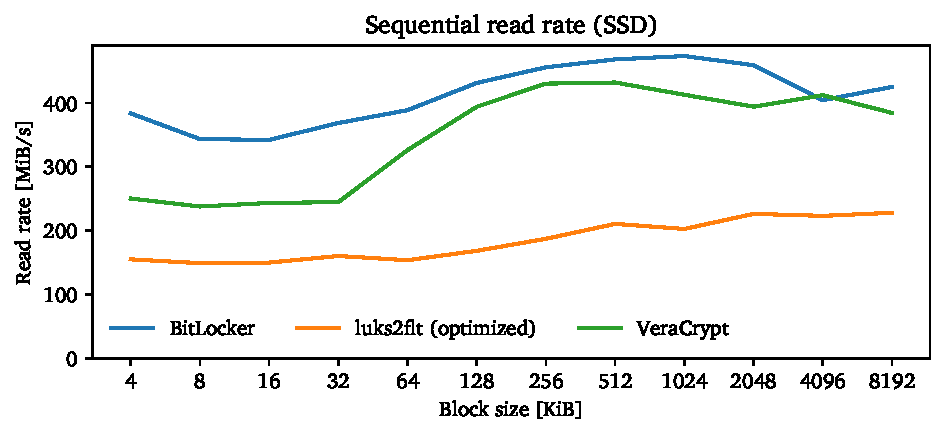
\includegraphics[scale=1]{../fig/performance.hwexperiments.optseq.pdf}
	\caption[
		Sequential read rates
	]{
		Sequential read rates. Each block size value is the average of three separate runs. Both the \texttt{iodepth} and \texttt{numjobs} parameters were set to a value of 1.
	}
	\label{fig:performance.hwexperiments.optseq}
\end{figure}

We observe the following:
\begin{itemize}[beginpenalty=10000]
	\item Except for a block size of 4096 KiB, where VeraCrypt has a 2\% higher rate, BitLocker always has the highest sequential read rate. It is up to 156.0\% higher than \texttt{luks2flt}'s (at 128 KiB), and up to 53.0\% higher than VeraCrypt's (at 4 KiB).
	\item BitLocker reaches its maximum at a block size of 1024 KiB, VeraCrypt at 512, \texttt{luks2flt} at 8192.
	\item \texttt{luks2flt} never reaches the performance of the other two drivers. BitLocker has an up to 156\% higher read rate (at 128 KiB), VeraCrypt up to 134\% (at 128 KiB).
\end{itemize}

\autoref{fig:performance.hwexperiments.optseq} contains the random-access read rates of the three drivers. BitLocker starts with a read rate of 19 MiB/s and, except for a dent at 4096 KiB, continually rises to a maximum of 335 MiB/s. \texttt{luks2flt}'s rate also begins at 19 MiB/s and steadily climbs to 195 MiB/s. VeraCrypt's rate at 4 KiB is 13 MiB/s, and then rises up to a value of 301 MiB/s at 8192 KiB. 

\begin{figure}[htb!]
	\center
	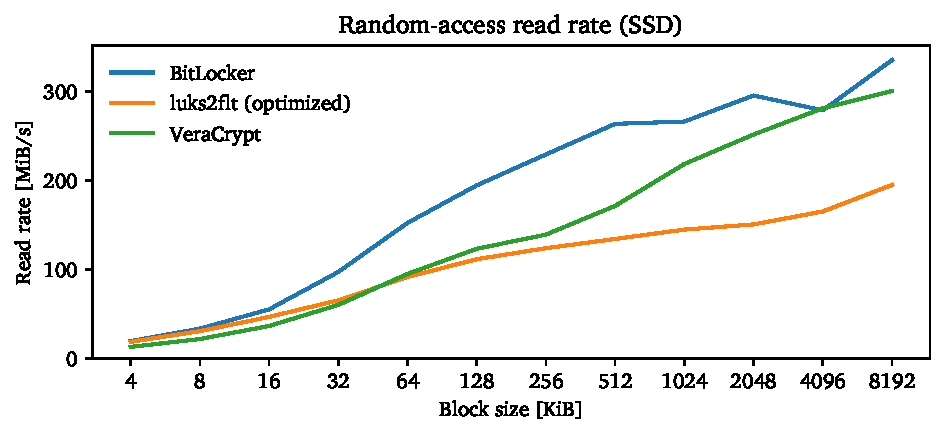
\includegraphics[scale=1]{../fig/performance.hwexperiments.optrand.pdf}
	\caption[
		Random-access read rates
	]{
		Random-access read rates. See \autoref{fig:performance.hwexperiments.optseq} for how we collected the data.
	}
	\label{fig:performance.hwexperiments.optrand}
\end{figure}

We observe the following:
\begin{itemize}[beginpenalty=10000]
	\item Except for a block size of 4096 KiB, where VeraCrypt has a 1\% higher rate, BitLocker always has the highest random-access read rate.
	\item For blocks smaller than 64 KiB, \texttt{luks2flt} has a higher random-access read rate than VeraCrypt. For large block sizes, the other two drivers have significantly higher read rates: BitLocker up to 96\% (at 512 KiB), VeraCrypt up to 70\% (at 4096 KiB).
\end{itemize}

\autoref{fig:performance.hwexperiments.optseqqueue} contains the sequential read rates of the three drivers with the \texttt{iodepth} parameter set to a value of 16. This means that \texttt{fio} submitted up to 16 I/O requests before waiting on the completion of requests. BitLocker's read rate starts at 344 MiB/s and, after a descent, rises to 521 MiB/s. VeraCrypt's read rate at 4 KiB is 241 MiB/s, and its maximum is 433 MiB/s at 8192. Its graph has a small dent from 1024 to 4096 KiB. \texttt{luks2flt} begins with a read rate of 149 MiB/s and rises to its maximum of 391 MiB/s at 4096 KiB.

\begin{figure}[htb!]
	\center
	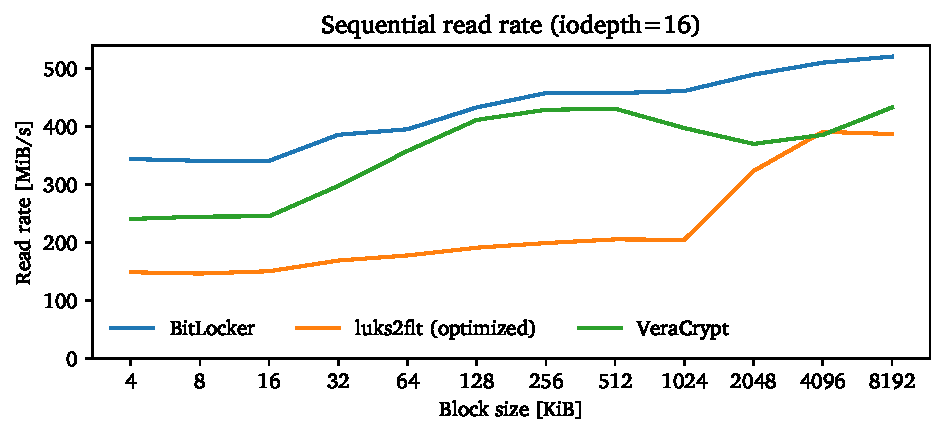
\includegraphics[scale=1]{../fig/performance.hwexperiments.optseqqueue.pdf}
	\caption[
		Sequential read rates with \texttt{iodepth=16}
	]{
		Sequential read rates with \texttt{iodepth=16}. Each block size value is the average of three separate runs. The \texttt{numjobs} parameter was set to a value of 1.
	}
	\label{fig:performance.hwexperiments.optseqqueue}
\end{figure}

We observe the following:
\begin{itemize}[beginpenalty=10000]
	\item BitLocker always has the highest sequential read rate, but in the range of 64 to 512 KiB blocks VeraCrypt's rate is relatively close to BitLocker's. At 8 KiB, BitLocker has a maximum read rate advantage over \texttt{luks2flt} of 133\%.
	\item At 4096 KiB, our driver has a slightly higher (1\%) read rate than VeraCrypt, but for smaller blocks, VeraCrypt is up to 116\% faster (at 256 KiB).
\end{itemize}

\autoref{fig:performance.hwexperiments.optseqqueue} shows the random-access read rates of the three drivers for an \texttt{iodepth} of 16. BitLocker's read rate at 4 KiB is 61 MiB/s. It rises continuously, although only very slowly for blocks larger than 256 KiB. Its maximum is 505 MiB/s at 8192 KiB. \texttt{luks2flt}'s rate starts at 58 MiB/s and rises more or less continuously until it reaches it maximum of 414 MiB/s. VeraCrypt begins with a rate of 25 MiB/s and climbs to its highest value of 364 MiB/s for the largest block size.

\begin{figure}[htb!]
	\center
	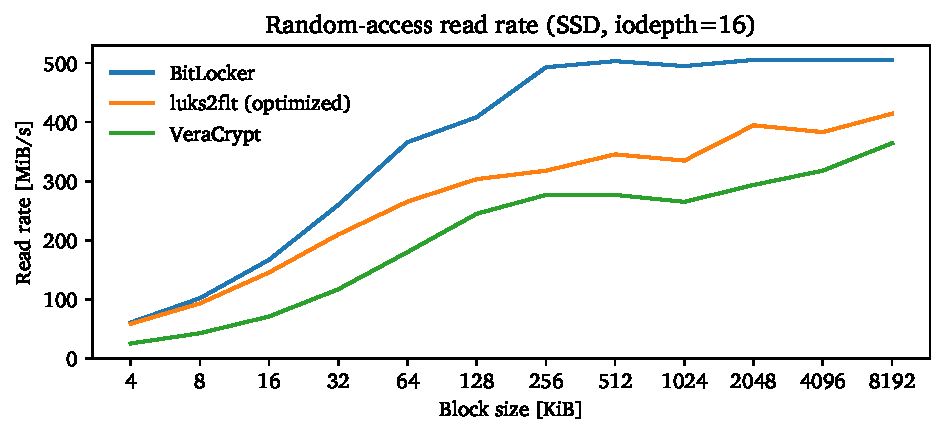
\includegraphics[scale=1]{../fig/performance.hwexperiments.optrandqueue.pdf}
	\caption[
		Random-access read rates with \texttt{iodepth=16}
	]{
		Random-access read rates with \texttt{iodepth=16}. See \autoref{fig:performance.hwexperiments.optseqqueue} for how we collected the data.
	}
	\label{fig:performance.hwexperiments.optrandqueue}
\end{figure}

We observe the following:
\begin{itemize}[beginpenalty=10000]
	\item BitLocker always has the highest random-access read rate, but for small block sizes our driver's rate is relatively close to BitLocker's. However, at 256 KiB BitLocker has a 55\% higher read rate compared to \texttt{luks2flt}, which is the highest advantage across all block sizes.
	\item \texttt{luks2flt} always has a higher read rate than VeraCrypt, up to a 133\% advantage (at 4 KiB).
\end{itemize}

\autoref{fig:performance.hwexperiments.optseqthreads} contains the sequential read rates of the three drivers with the \texttt{numjobs} parameter set to a value of 16. This means that 16 threads concurrently executed the same job. BitLocker begins with a read rate of 107 MiB/s, which, with a small dent at 32 KiB, climbs to its maximum of 492 MiB/s at 512 KiB. It then falls back down to 187 MiB/s at 8192 KiB. VeraCrypt's read rate starts at 146 MiB/s, then jaggedly rises to a maximum of 431 MiB/s at 256 KiB, then also jaggedly goes back down to 253 MiB/s. Our driver's read rate for 4 KiB blocks is 106 MiB/s, and, with some fluctuations, it climbs to its maximum value of 211 MiB/s at 1024 KiB. It then slowly falls back down to 170 MiB/s.

\begin{figure}[htb!]
	\center
	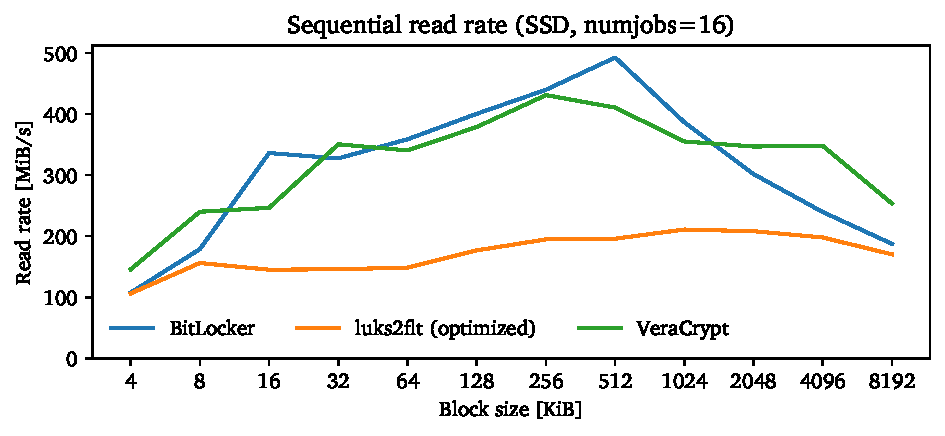
\includegraphics[scale=1]{../fig/performance.hwexperiments.optseqthreads.pdf}
	\caption[
		Sequential read rates with \texttt{numjobs=16}
	]{
		Sequential read rates with \texttt{numjobs=16}. Each block size value is the average of three separate runs, with the value used for each run being the average read rate of all threads. The \texttt{iodepth} parameter was set to a value of 1.
	}
	\label{fig:performance.hwexperiments.optseqthreads}
\end{figure}

We observe the following:
\begin{itemize}[beginpenalty=10000]
	\item VeraCrypt and BitLocker both have the highest sequential read rate for respectively six of the twelve tested block sizes.
	\item VeraCrypt reaches its maximum rate at 256 KiB, BitLocker at 512, our driver at 1024.
	\item Both other drivers perform significantly better than \texttt{luks2flt} for most block sizes. BitLocker has an up to 151\% higher rate (at 512 KiB), VeraCrypt up to 140\% (at 32 KiB).
\end{itemize}

\autoref{fig:performance.hwexperiments.optrandthreads} shows the three drivers' random-access read rates for multi-threaded job execution. BitLocker's read rate starts at 32 MiB/s, reaches its maximum at 25 KiB with a value of 294 MiB/s, and then goes back down to 236 MiB/s. \texttt{luks2flt}'s rate begins at 32 MiB/s, has its maximum value of 220 MiB/s at 256 KiB, and, with a dent at 1024 KiB, slowly decreases to 212 MiB/s at 8192 KiB. The VeraCrypt driver's read rate is 19 MiB/s for 4 KiB blocks and a maximum of 203 MiB/s for 256 KiB blocks. After a dent in the range from 512 to 4096 KiB, its rate for 8192 KiB is 201 MiB/s.

\begin{figure}[htb!]
	\center
	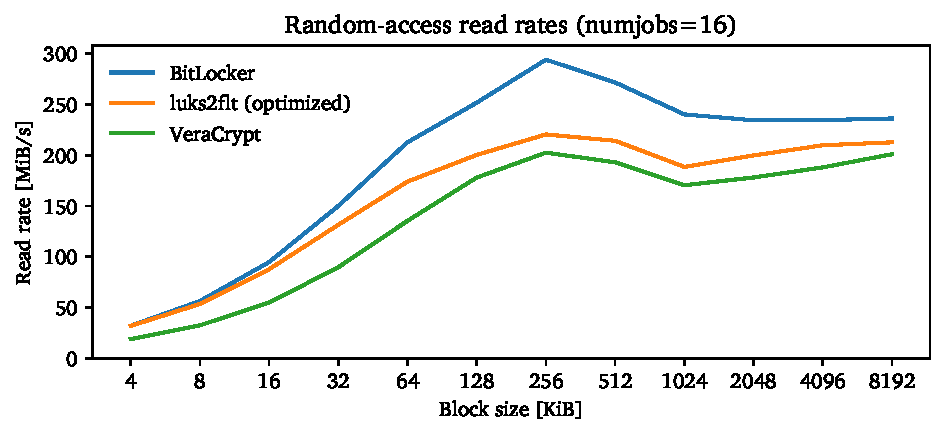
\includegraphics[scale=1]{../fig/performance.hwexperiments.optrandthreads.pdf}
	\caption[
		Random-access read rates with \texttt{numjobs=16}
	]{
		Random-access read rates with \texttt{numjobs=16}. See \autoref{fig:performance.hwexperiments.optseqthreads} for how we collected the data.
	}
	\label{fig:performance.hwexperiments.optrandthreads}
\end{figure}

We observe the following:
\begin{itemize}[beginpenalty=10000]
	\item BitLocker is always the fastest driver, with an up to 33\% higher random-access read rate than luks2flt (at 256 KiB), and up to 74.0\% higher than VeraCrypt (at 8 KiB).
	\item All drivers reach their respective maximum rate at a block size of 256 KiB.
	\item \texttt{luks2flt} always has a higher read rate than VeraCrypt, with an up to 69\% advantage (at 4 KiB).
\end{itemize}

\autoref{fig:performance.hwexperiments.optseqthreadsqueue} shows the tested drivers' sequential read rates for multi-thread job execution with an \texttt{iodepth} of 16. BitLocker starts with a read rate of 131 MiB/s, which then grows to 395 MiB/s for 32 KiB blocks. It then jaggedly decreases to 328 MiB/s at 4096 KiB, and finally falls down to 87 MiB/s. VeraCrypt's rate begins at 128 MiB/s, rises to 404 MiB/s at 32 KiB, and, after a dent at 64 KiB, slowly decreases to 317 MiB/s at 4096 KiB. The read rate at 8192 KiB is 90 MiB/s. \texttt{luks2flt}'s read rate starts at 132 MiB/s, rises mostly continuously to 275 MiB/s at 4096 KiB, and then falls down to 38 MiB/s at 8192 KiB.

\begin{figure}[htb!]
	\center
	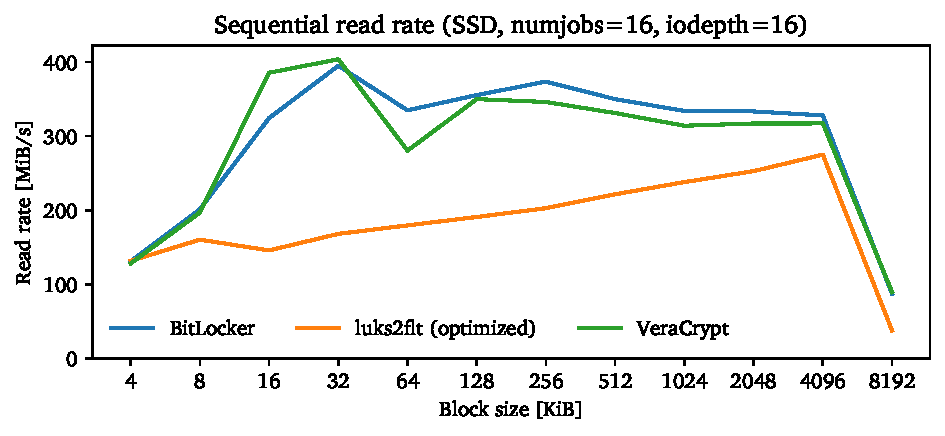
\includegraphics[scale=1]{../fig/performance.hwexperiments.optseqthreadsqueue.pdf}
	\caption[
		Sequential read rates with \texttt{numjobs=16} and \texttt{iodepth=16}
	]{
		Sequential read rates with \texttt{numjobs=16} and \texttt{iodepth=16}. Each block size value is the average of three separate runs, with the value used for each run being the average read rate of all threads.
	}
	\label{fig:performance.hwexperiments.optseqthreadsqueue}
\end{figure}

We observe the following:
\begin{itemize}[beginpenalty=10000]
	\item Except for 16, 32, and 8192 KiB blocks, where VeraCrypt is the fastest, BitLocker has the highest sequential read rate. Compared to our driver, BitLocker has an up to 135\% advantage (at 32 KiB), and VeraCrypt has an up to 165\% higher rate (at 16 KiB).
	\item BitLocker and VeraCrypt have their respective maximum read rates at 32 KiB, \texttt{luks2flt} at 4096.
	\item All drivers' read rates suddenly plummet down at 8192 KiB.
\end{itemize}

\autoref{fig:performance.hwexperiments.optrandthreadsqueue} has the random-access read rates for multi-thread job execution with an \texttt{iodepth} of 16. BitLocker's read rate starts at 31 MiB/s and rises to its maximum of 241 MiB/s at 4096 KiB, although only slowly starting from a block size of 256 KiB. \texttt{luks2flt} has a rate of 31 MiB at 4 KiB, which then rises to a maximum of 222 MiB/s at 4096 KiB, with a dent at 1024 and 2048 KiB. VeraCrypt starts with a read rate of 19 MiB/s, which mostly continuously grows to its maximum of 202 MiB/s at 8192 KiB.

\begin{figure}[htb!]
	\center
	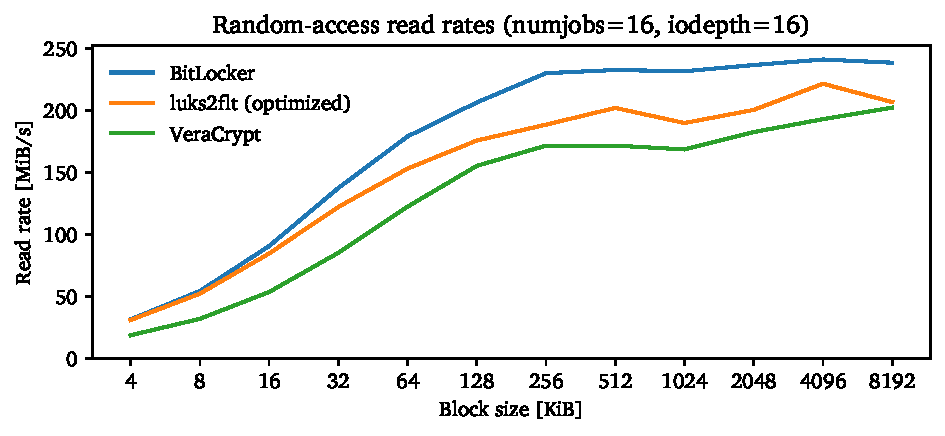
\includegraphics[scale=1]{../fig/performance.hwexperiments.optrandthreadsqueue.pdf}
	\caption[
		Random-access read rates with \texttt{numjobs=16} and \texttt{iodepth=16}
	]{
		Random-access read rates with \texttt{numjobs=16} and \texttt{iodepth=16}. See \autoref{fig:performance.hwexperiments.optseqthreadsqueue} for how we collected the data.
	}
	\label{fig:performance.hwexperiments.optrandthreadsqueue}
\end{figure}

We observe the following:
\begin{itemize}[beginpenalty=10000]
	\item BitLocker always has the highest random-access read rate, with an up to 22\% advantage over our driver (at 256 KiB) and a 70\% advantage over VeraCrypt (at 8 KiB).
	\item \texttt{luks2flt} always has a higher read rate than VeraCrypt, with an up to 66\% advantage (at 4 KiB).
\end{itemize}

\paragraph{Discussion}
Combining our observations from all measurements, we close with the following thoughts:
\begin{itemize}[beginpenalty=10000]
	\item In almost all cases, BitLocker has the highest read rate, regardless of the access pattern. As already detailed in \autoref{chap:performance.vmexperiments}, this is not really surprising, because it is not a fair comparison. Nonetheless, from time to time VeraCrypt's sequential read rate is quite close to BitLocker's, and our driver's multi-threaded random-access read rate can almost keep up with BitLocker's.
	\item Regrettably, the disabled optimization options led to a performance regression. Comparing the measurements with the same parameters (i.e. \texttt{iodepth=1} and \texttt{numjobs=1}), we can see that on real hardware \texttt{luks2flt} cannot compete with VeraCrypt as well as in the virtual machine. This is the case for both sequential and random access.
	\item Our driver's sequential read rate is consistently lower than that of the other two drivers. As discussed in the previous section, VeraCrypt probably has better sequential performance because of its read ahead caching. The maximum advantage the other drivers have over \texttt{luks2flt} mostly lies between 130\% and 150\%. However, when at least one of the \texttt{iodepth} or \texttt{numjobs} parameter has a value of 16, \texttt{luks2flt} can almost catch up with one of the other drivers for large block sizes.
	\item Even though \texttt{luks2flt} cannot compete at random access when only one I/O request is sent at a time (at least not for large block sizes), the situation looks differently for \texttt{iodepth=16} and/or \texttt{numjobs=16}: here, our driver always has a higher read rate than VeraCrypt, and even BitLocker has an at most 55\% higher rate. BitLocker as a proprietary driver is out of reach for theorizing. However, we have a suspicion why VeraCrypts manages multiple requests at the same time not as well as \texttt{luks2flt}: every read request has to pass through three queues (Main, I/O, and Completion), and every queue only has one thread working on its requests. \cite{Korchagin2020} showed that removing some queues in \texttt{dm-crypt} can lead to significant read rate improvements, and that may be the case for VeraCrypt, too.
	\item In the last section, we noted that VeraCrypt's sequential read rate peaked at 256 KiB blocks. We also highlighted that this was the size of the fragments that larger blocks get broken up into. In this section's measurements, this generally was also the case: VeraCrypt's sequential read rate either peaked at a block size of 256 or 512 KiB or did not improve by much for larger blocks.
\end{itemize}

\subsection{Measuring Read Rates over Time}
\label{chap:performance.hwexperiments.readrateovertime}
\texttt{fio} comes with an option to enable the logging of current read rates, \texttt{write\_bw\_log}. By default, one entry in the log file corresponds to one completed I/O request. This is not what we wanted for two reasons: firstly, this does not scale well with larger block sizes, as there are fewer I/O operations when using larger blocks; and secondly, we are not interested in single I/O requests, but the general trend over time (the logs with one line per completed request contain large read rate spikes which we do not care about). Fortunately, there is also an option to log the average bandwidth of the last $N$ milliseconds, where the value of $N$ is configurable: \texttt{log\_avg\_msec}. We found that 32 ms is a good value for this option, yielding data with reasonable high time resolution, but not too much spikes from the completion of individual I/O requests.

Note that all measurements in this section are values of single runs, and not averages of three runs of the same job like in the section before.

\paragraph{Results and Observations}
\autoref{fig:performance.hwexperiments.seqovertime} shows how BitLocker's, VeraCrypt's, and \texttt{luks2flt}'s read rates behave over time for a block size of 32 KiB. BitLocker's rate mostly stays between 367 and 375 MiB/s, with two short sections where it is between 375 and 383 MiB/s and some spikes, mostly downward. VeraCrypt's read rate generally falls between 226 and 290 MiB/s, but heavily fluctuates in that range. Except for the first 2.5 seconds, where it fluctuates between 149 and 169 MiB/s, \texttt{luks2flt}'s rate mostly stays between 161 and 173 MiB/s.

\begin{figure}[htb!]
	\center
	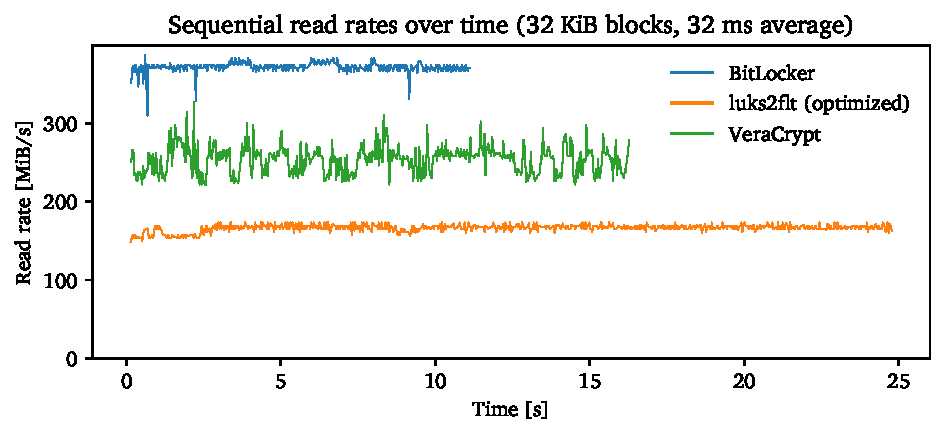
\includegraphics[scale=1]{../fig/performance.hwexperiments.seqovertime.pdf}
	\caption[
		Sequential read rates over time
	]{
		Sequential read rates over time. We used a block size of 32 KiB and set \texttt{fio}'s \texttt{log\_avg\_msec} parameter to 32 ms. The \texttt{iodepth} was set to a value of 1.
	}
	\label{fig:performance.hwexperiments.seqovertime}
\end{figure}

\autoref{fig:performance.hwexperiments.seqovertimebox} shows the distribution of the read rates from \autoref{fig:performance.hwexperiments.seqovertime} in a box plot. The median of BitLocker's read rate is 372 MiB/s, the lower quartile is 370 MiB/s, and the upper quartile is 375 MiB/s. The whiskers are at 363 and 382 MiB/s, and there are some outliers between 310 and 387 MiB/s. Our driver's median rate is 166 MiB/s, its lower quartile is 165 MiB/s, and its upper quartile is 169 MiB/s. The whiskers are at 160 and 174 MiB/s, and there are some outliers in the 149 to 159 MiB/s range. The median rate of VeraCrypt is 256 MiB/s, the lower quartile is 238 MiB/s, and the upper quartile is 262 MiB/s. The whiskers are at 221 and 298 MiB/s, and there are some outliers between 300 and 327 MiB/s.

\begin{figure}[htb!]
	\center
	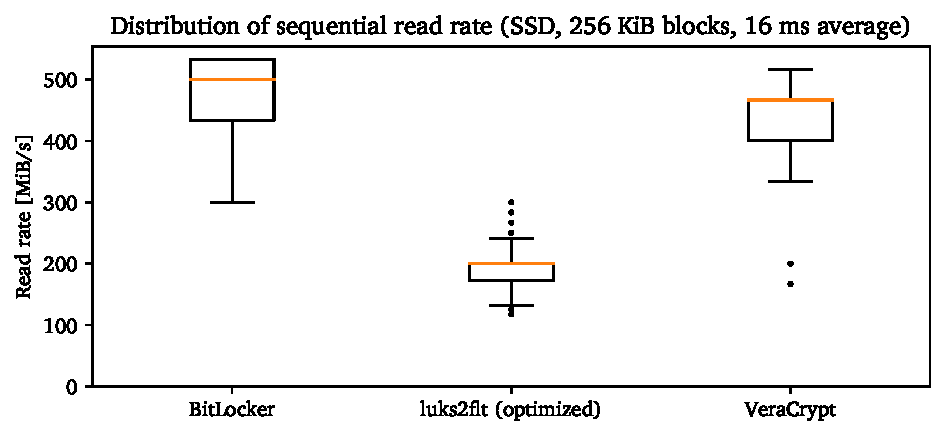
\includegraphics[scale=1]{../fig/performance.hwexperiments.seqovertimebox.pdf}
	\caption[
		Distribution of sequential read rates over time
	]{
		Distribution of sequential read rates over time. This is a different visualization of the data presented in \autoref{fig:performance.hwexperiments.seqovertime}.
	}
	\label{fig:performance.hwexperiments.seqovertimebox}
\end{figure}

We observe the following:
\begin{itemize}[beginpenalty=10000]
	\item BitLocker has the highest sequential read rate, VeraCrypt comes second, and our driver comes third.
	\item \texttt{luks2flt} has the least variation in read rate values. Bitlocker comes close, but its outliers are further away from the mean. VeraCrypt's read rate has significantly more variation over time than the other drivers'.
\end{itemize}

\autoref{fig:performance.hwexperiments.randovertime} shows the drivers' random-access read rates over time. BitLocker's read rates switches between lying in the 98 to 100 MiB/s range and the 94 to 96 MiB/s range, with some mostly downward spikes. \texttt{luks2flt} has a read rate that concentrates around either 64 MiB/s or 69 MiB/s, with some spikes in both directions. VeraCrypt's rate generally oscillates around 61 MiB/s, with exceptions, mostly at the beginning and the end of the run.

\begin{figure}[htb!]
	\center
	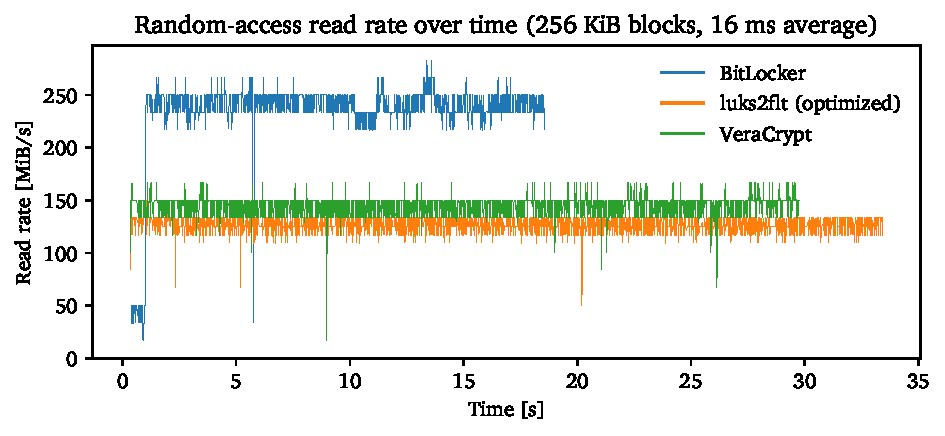
\includegraphics[scale=1]{../fig/performance.hwexperiments.randovertime.pdf}
	\caption[
		Random-access read rates over time
	]{
		Random-access read rates over time. See \autoref{fig:performance.hwexperiments.seqovertime} for how we collected the data.
	}
	\label{fig:performance.hwexperiments.randovertime}
\end{figure}

\autoref{fig:performance.hwexperiments.randovertimebox} shows the distribution of the read rates from \autoref{fig:performance.hwexperiments.randovertime}. BitLocker's median read rate is 99 MiB/s, the lower quartile is 95 MiB/s, and the upper quartile is 99 MiB/s. The whiskers are at 91 and 101 MiB/s. The 69 to 113 MiB/s range contains all outliers, except for one at 35 MiB/s. The median of \texttt{luks2flt}'s read rate is 65 MiB/s, the lower quartile is 64 MiB/s, and the upper quartile is 69 MiB/s. The whiskers are at 57 and 75 MiB/s, and there are some outliers between 44 and 80 MiB/s. VeraCrypt has a median rate of 61 MiB/s, with the lower quartile being 60 MiB/s and the upper quartile being 61 MiB/s. The whiskers are at 57 and 75 MiB/s, and there are some outliers in the 32 to 71 MiB/s range.

\begin{figure}[htb!]
	\center
	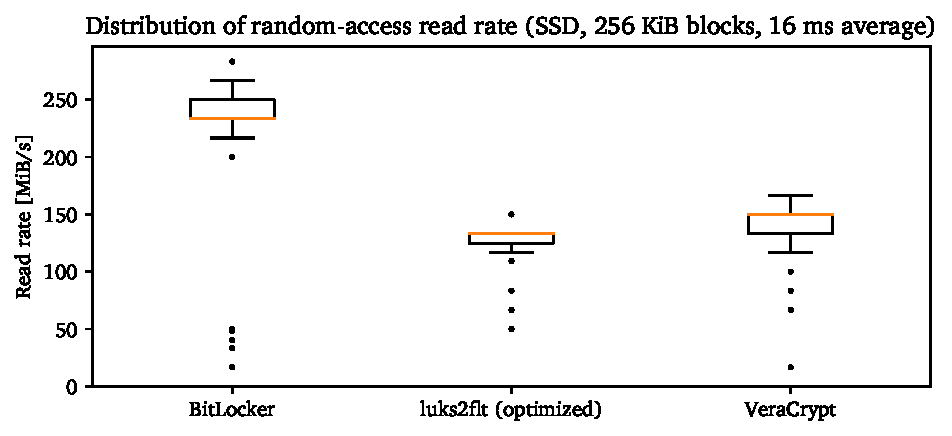
\includegraphics[scale=1]{../fig/performance.hwexperiments.randovertimebox.pdf}
	\caption[
		Distribution of random-access read rates over time
	]{
		Distribution of random-access read rates over time. This is a different visualization of the data presented in \autoref{fig:performance.hwexperiments.randovertime}.
	}
	\label{fig:performance.hwexperiments.randovertimebox}
\end{figure}

We observe the following:
\begin{itemize}[beginpenalty=10000]
	\item BitLocker has the highest radnom-access read rate, our driver comes second, and VeraCrypt closely follows behind.
	\item VeraCrypt's read rate has the least variation, and BitLocker's and \texttt{luks2flt}'s both alternate between two small ranges. The rates of all three drivers contain occasional outliers.
\end{itemize}

We also looked at other block sizes than 32 KiB (all that we tested in the last section), and found this general trend: the larger the blocks, the more variations in the read rate (i.e. the boxes and whiskers stretched out farther, and there were also less outliers). We chose to display the graphs for 32 KiB blocks because they seemed a good compromise between being neither completely on one end of the block size range nor too jagged.

\paragraph{Discussion}
Combining our observations, we close with the following thoughts:
\begin{itemize}[beginpenalty=10000]
	\item The read rates in our measurements match what we saw in the last section (see \autoref{fig:performance.hwexperiments.optseq} and \autoref{fig:performance.hwexperiments.optrand}).
	\item VeraCrypt had the most variation in read rate for sequential reading, and the least for random-access reading. Looking at our measurements over time for other block rates however we could not find a general trend; no driver regularly showed more or less variation in read rate than the others. However, these were all measurements of single runs. To find or rule out trends with more certainty, measurements from multiple runs should be combined.
	\item The trend that higher block sizes lead to more variation in the read rate probably occurs because the completion of a single I/O request has more impact on the short-time read rate the bigger the read block is.
\end{itemize}